
\chapter{Motion in One Dimension and SUVAT}
\label{sec: motion in 1D}
\section{Mechanics}
Throughout this course we will study objects in motion. This could be a ball rolling down a hill, a spring oscillating up and down, or a pendulum. The first part of this course is focussed on \textbf{kinematics}, the study of how objects move. Later in the module we will also deal with \textbf{dynamics}, the study of why objects move. These are both subsets of \textbf{mechanics}, the study of moving objects. \\


\begin{figure}[ht]
    \centering
    
    {\displaymathother
    \ThisAltText{ This is a diagram of a ball rolling down a hill}
    %\pdftooltip{ 
   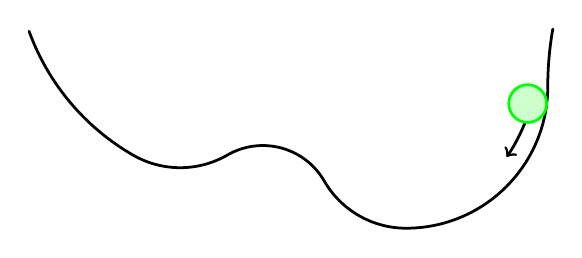
\begin{tikzpicture}[line width=1pt,line cap=round,line join=round,x=6mm,y=6mm]
\draw (5,0) arc(0:-90:3) arc(-90:-150:2) arc(30:120:1.5) arc(-60:-120:2) arc(-120:-160:5);
\draw (5,0) arc(180:170:7);
\draw[->,shorten <=7] ({2+2.6*cos(-8)},{2.6*sin(-8)}) arc(-8:-35:2.6);
\draw[green,fill=green!20!white] ({2+2.6*cos(-8)},{2.6*sin(-8)}) circle (0.4);
\end{tikzpicture}
}
   % }{A ball rollling down a hill.}
    \caption{A ball rolling down a hill.}
    \label{fig: ball on a hill}
\end{figure}

Kinematics is concerned with quantities like:
\begin{itemize}
\setlength{\itemsep}{-5pt}
    \item \textbf{Displacement:} The distance an object moves in a given direction, typically measured in metres or similar units.
    \item \textbf{Distance:} How far an object has moved without keeping track of the direction. We use the symbol $s$ for displacement.
    \item \textbf{Speed:} The rate of change of distance with respect to time.
    \item \textbf{Velocity:} The rate of change of displacement with respect to time, e.g. the speed in a given direction. Velocity is usually measured in metres per second, m/s or $\text{ms}^{-1}$. we use the symbols $v$ or $u$ for velocity. When the velocity is constant it is related to the displacement through $v=\frac{s}{t}$, i.e velocity is displacement divided by time.
    \item \textbf{Acceleration:} The rate of change of velocity with respect to time, usually measured in metres per second squared, $\text{m/}\text{s}^{2}$ or $\text{ms}^{-2}$. Acceleration is given the symbol a.
\end{itemize}

The formula relating constant velocity, displacement, and time can be recalled using the formula triangle in \cref{fig: vst triangle}.\\

\begin{figure}[ht]
    \centering
  {\displaymathother
    \ThisAltText{ The formula triangle for displacement, velocity, and time.}
     % \pdftooltip{ 
   \Huge {\formulatriang[.4]{$s$}{}{$v$}{}{$t$}{}}
   }
   %}{The formula triangle for velocity, displacement, and time.}
    \caption{The formula triangle for constant velocity, displacement, and time. To use the triangle cover up the quantity that you want to calculate and you are left with the formula for it. For example if $s$ is covered up we are left with $v\times t$}
    \label{fig: vst triangle}
\end{figure}


Speed and distance are examples of scalars. Quantities that have a size (also called a magnitude) but not a direction. While velocity, displacement, and acceleration are vectors. This means that they have both a size and a direction.\\

The distinction between scalars and vectors is an important one and we will make a lot of use of both quantities repeatedly during this module.



\section{Motion in 1D}
The easiest way to remember the difference is to think about motion along a line in one dimension.\\

\begin{figure}[ht]
    \centering
    %\pdftooltip{
    \ThisAltText{ A one dimensional line signifying the x-axis.}
    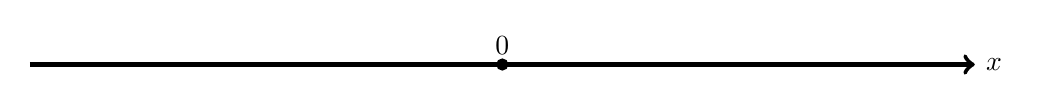
\begin{tikzpicture}
\draw[black, ultra thick,->] (-6,0) --(6,0) node[anchor=west]{$x$};
\filldraw[black] (0,0) circle (2pt) node[anchor=south]{0};
\end{tikzpicture}
%}{A schematic of the x-axis }
    \caption{A one dimensional line described by the coordinate x. The point $x=0$ is marked in the middle of the line with $x$ negative to the left of this and positive to the right.}
    \label{fig: x-axis fig}
\end{figure}

The line shown in \cref{fig: x-axis fig} is known as the $x$-axis since the value of $x$ tells us how far along the line we are. In \cref{fig: x-axis fig2} we have two marked points, $x_{1}$ and $x_{2}$ on the $x$-axis. If we think of an object starting at $x_{1}$ and moving to $x_{2}$ then the displacement is the change\footnote{In physics we often use the notation $\Delta$ to mean the change in a quantity.} in position $\Delta x =x_{2}-x_{1}$.\\

The difference between displacement and distance is that the distance is always positive, while the displacement is positive when an object is moving to the right and negative for an object moving to the left.\\

\begin{figure}[ht]
    \centering
    \ThisAltText{ The x-axis with two points marked showing where the object is moving between.}
   % \pdftooltip{
   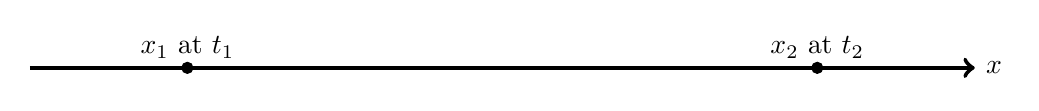
\begin{tikzpicture}
\draw[black, ultra thick,->] (-6,0) --(6,0) node[anchor=west]{$x$};
\filldraw[black] (-4,0) circle (2pt) node[anchor=south]{$x_{1}$ at $t_{1}$};
\filldraw[black] (4,0) circle (2pt) node[anchor=south]{$x_{2}$ at $t_{2}$};
\end{tikzpicture}
%}{A schematic of the x-axis with two points marked }
    \caption{The $x$-axis with two points marked, $x_{1}$ and $x_{2}$, where the moving object is at the times $t_{1}$ and $t_{2}$.}
    \label{fig: x-axis fig2}
\end{figure}

The \textbf{sign} of $\Delta x$, either positive or negative is the direction, it shows if the object is moving to the right or to the left. Note that the distance the object travels is given by $\vert \Delta x\vert$, the modulus of $\Delta x$.\\

We can explicitly see the difference between distance and displacement if we consider the following two examples:
\begin{itemize}
\setlength{\itemsep}{-5pt}
    \item if $x_{1}=0$ and $x_{2}=2$ then the displacement is $\Delta x=2-0=2$ and the distance is also $2$.
    \item If $x_{1}=0$ and $x_{2}=-2$ then the displacement is $\Delta x = -2-0=-2$ while the distance is still $2$.
\end{itemize}
So the distance does not care whether we move left or right along the $x$-axis, while the displacement cares about the difference.\\

The \textbf{average velocity} is the displacement divided by the difference between the time when the object is at $x_{2}$ and the time at $x_{1}$,
\begin{equation}
    v_{\text{avg}}=\frac{\Delta x}{\Delta t}=\frac{x_{2}-x_{1}}{t_{2}-t_{1}}.
    \label{eq: average velocity}
\end{equation}
You may recognise this as the formula for the gradient of a straight line starting at $(t_{1},x_{1})$ and ending at $(t_{2},x_{2})$. In fact plotting displacement against time is a convenient way to visualise an objects motion. In \cref{fig: displacement time graph 1} we see two examples of this type of plot, in red we have the case of constant velocity, while in blue we see that the velocity is changing.\\

\begin{figure}[ht]
    \centering
    \ThisAltText{ A displacement time graph for constant velocity motion, a straight line, and changing velocity.}
   % \pdftooltip{
   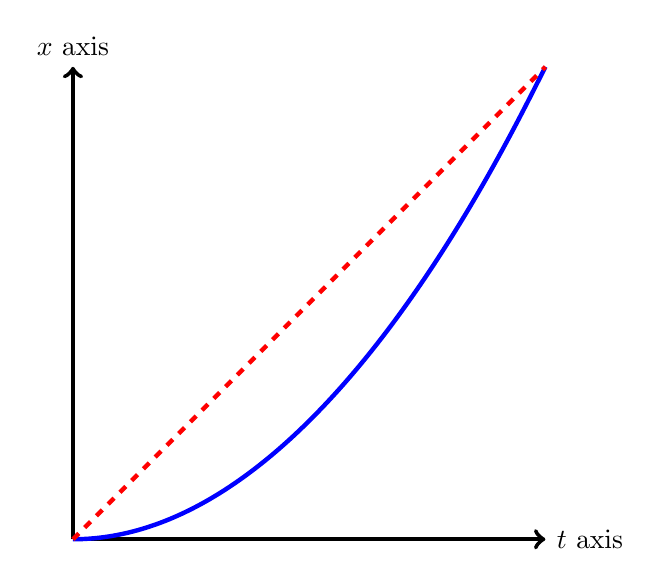
\begin{tikzpicture}
\draw[black, ultra thick,->] (0,0) --(6,0) node[anchor=west]{$t$ axis};
\draw[black, ultra thick,->] (0,0) --(0,6) node[anchor=south]{$x$ axis};
%\draw[step=1cm,gray,very thin] (-2,-2) grid (6,6);
\draw[blue, ultra thick] (0,0) parabola (6,6);
\draw[red, ultra thick, dashed] (0,0) -- (6,6);
% \filldraw[black] (-4,0) circle (2pt) node[anchor=south]{$x_{1}$ at $t_{1}$};
% \filldraw[black] (4,0) circle (2pt) node[anchor=south]{$x_{2}$ at $t_{2}$};
\end{tikzpicture}
%}{A displacement time graph showing the difference between constant velocity motion and motion with a changing velocity.}
    \caption{A displacement time graph showing the difference between constant velocity motion, in red and dashed, and motion with a changing velocity, in blue.}
    \label{fig: displacement time graph 1}
\end{figure}

To read this off the graphs notice that in the constant velocity case no matter which points on the $x$-axis we think of starting and ending at, when we use \cref{eq: average velocity} we will find the same value. This is why we called it the constant velocity case. The velocity is the gradient, rate of change, of a displacement time graph, and a straight line has a constant gradient.\\

For the second case, the blue curve\footnote{Mathematically the blue curve is known as a parabola and is described by a formula $x=t^{2}$ so we can also compute its gradient at any point.}, the gradient is not constant it changes from point to point along the curve. In this case \cref{eq: average velocity} for the average velocity will only be an approximation to the gradient of the curve. This approximation will get better and better as the time difference between the two points, $\Delta t$, gets smaller. To get the instantaneous velocity we would need to take $\Delta t$ to zero, and then the velocity $v$ is given by the \textbf{derivative} of $x$,
\begin{equation*}
    v=\frac{\ud x}{\ud t}.
\end{equation*}
In this module we are not assuming any familiarity with calculus so will not need to use the derivative to calculate the velocity. 

\begin{figure}[ht]
    \centering
    %\pdftooltip{
    \ThisAltText{ A displacement time graph showing an object moving away from its initial position before turning around and returning.}
    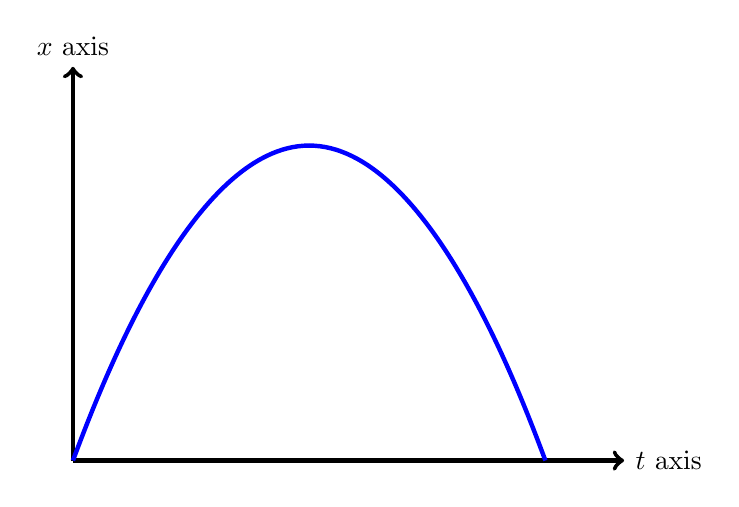
\begin{tikzpicture}
\draw[black, ultra thick,->] (0,0) --(7,0) node[anchor=west]{$t$ axis};
\draw[black, ultra thick,->] (0,0) --(0,5) node[anchor=south]{$x$ axis};
%\draw[step=1cm,gray,very thin] (-2,-2) grid (7,7);
\draw[blue, ultra thick] (3,4) parabola (6,0);
\draw[blue, ultra thick] (3,4) parabola (0,0);
% \filldraw[black] (-4,0) circle (2pt) node[anchor=south]{$x_{1}$ at $t_{1}$};
% \filldraw[black] (4,0) circle (2pt) node[anchor=south]{$x_{2}$ at $t_{2}$};
\end{tikzpicture}
%}{A displacement time graph where the object returns to its starting position.}
    \caption{A displacement time graph where the object returns to its starting position. This is the sort of graph we will see when looking at objects falling under gravity next week.}
    \label{fig: displacement time graph 2}
\end{figure}

When the velocity is constant we can just use \cref{eq: average velocity} and the equation triangle in \cref{fig: vst triangle} to relate velocity, displacement, and time. If the velocity is changing in time we need to consider the acceleration. This is easiest to understand if we visualise the changing velocity on a velocity time graph. This is just like the displacement time graphs that we saw above but we plot the velocity of the object on the vertical axis rather than the displacement.\\

\begin{figure}[ht]
    \centering
   % \pdftooltip{
   \ThisAltText{ A velocity time graph showing uniform motion where the velocity follows a straight line.}
   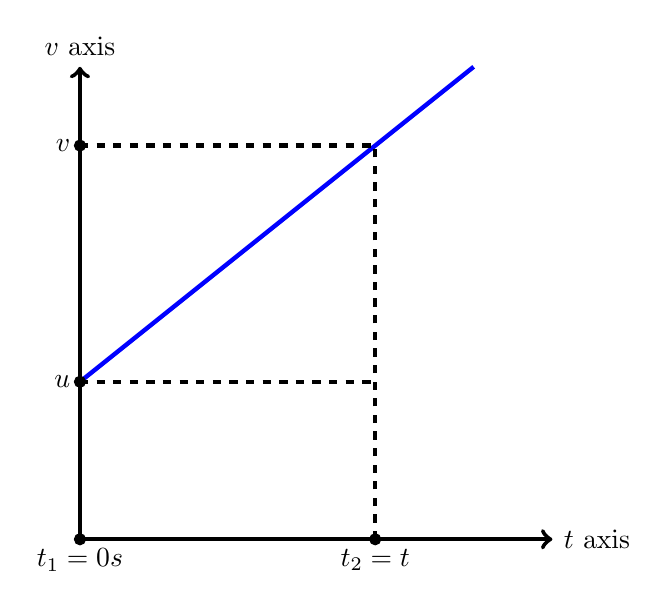
\begin{tikzpicture}
\draw[black, ultra thick,->] (0,0) --(6,0) node[anchor=west]{$t$ axis};
\draw[black, ultra thick,->] (0,0) --(0,6) node[anchor=south]{$v$ axis};
%\draw[step=1cm,gray,very thin] (-2,-2) grid (6,6);
%\draw[blue, ultra thick] (0,0) parabola (6,6);
\draw[blue, ultra thick] (0,2) -- (5,6);
\filldraw[black] (0,2) circle (2pt) node[anchor=east]{$u$};
\filldraw[black] (0,5) circle (2pt) node[anchor=east]{$v$};
\draw[black, ultra thick, dashed] (0,5) --(3.75,5);
\draw[black, ultra thick, dashed] (0,2) --(3.75,2);
\draw[black, ultra thick, dashed] (3.75,0) --(3.75,5);
\filldraw[black] (3.75,0) circle (2pt) node[anchor=north]{$t_{2}=t$};
\filldraw[black] (0,0) circle (2pt) node[anchor=north]{$t_{1}=0\text{s}$};
\end{tikzpicture}
%}{A velocity time graph showing uniform motion.}
    \caption{A velocity time graph showing uniform motion starting with velocity $u$ at time zero and accelerating to have velocity $v$ at time $t_{2}$.}
    \label{fig: velocity time graph 1}
\end{figure}

Consider the motion shown in \cref{fig: velocity time graph 1}, here the moving object has the initial velocity $u$ at time $t_{1}=0\text{s}$ which changes to the final velocity $v$ at time $t_{2}=t$. The acceleration is the rate of change of velocity so the average acceleration is given by
\begin{equation}
    a_{\text{avg}}=\frac{\Delta v}{\Delta t}=\frac{v-u}{t}.
    \label{eq: average acceleration}
\end{equation}

As with velocity, if the acceleration is changing then the instantaneous acceleration will be different from the average acceleration and we would need calculus to compute it properly. In this module we will rarely go beyond the case of constant acceleration\footnote{We will only need this when discussing circular motion later in the module. and there we will describe the acceleration in a slightly different way which avoids using the derivative.}. This is called \textbf{uniform motion}.\\

For uniform motion we can rearrange \cref{eq: average acceleration} to make the final velocity $v$ the subject:
\begin{equation}
    v=u+at.
    \label{eq: Kinematic equation 1}
\end{equation}
This is the first of the so called \textbf{Kinematic equations} that we have met. These are the equations relating velocity, time, acceleration, and displacement, by the end of this module you will be very familiar with using these kinematic equations to solve problems. 

\paragraph{Example 2.1:} A car is travelling at $8\text{m/s}$ and breaks for $6\text{s}$  to reduce its velocity to $2\text{m/s}$ calculate its deceleration.

First collect together what we know about the problem:
\begin{itemize}
\setlength{\itemsep}{-5pt}
    \item initial velocity is $u=8\text{m/s}$
    \item final velocity is $v=2\text{m/s}$
    \item time is $t=6\text{s}$.
\end{itemize}
We know that we are in the realm of uniform motion so can use $a=\frac{v-u}{t}$ to find the acceleration. substituting in the numbers gives:
\begin{align*}
    a&=\frac{v-u}{t}=\frac{2-8}{6}=-\frac{6}{6}=-1\frac{\text{m}}{\text{s}^{2}}.
\end{align*}
The negative sign shows that the car is decelerating and is because the velocity is decreasing. Note that it is very important to always include the units in your final answer.\\

\vspace{2cm}

\section{Kinematic Equations}
There are several other kinematic equations that will be useful, deciding which one to use to solve a given problem is something that you will learn by practising solving problems. In the exam you will be given a formula book that will have most of the equations in it. The formula included in the formula sheet are given at the end of these lecture notes.\\

For completeness we will derive the other kinematic equations here and use them to solve an example. \textbf{You do not need to be able to replicate the derivations, but you do need to know how to use the equations.}\\

The formula above, \cref{eq: average acceleration}, is good if we know any three of initial velocity, final velocity, acceleration, and time. However, often we will be interested in the displacement of an object during its motion. This means that we need a way to calculate displacement in terms of the other quantities.  Let us start with what we know. For an object in uniform motion we have that:
\begin{itemize}
\setlength{\itemsep}{-5pt}
    \item The acceleration is related to the initial velocity, final velocity, and the time the object is moving for through
    \begin{equation*}
        v=u+at.
    \end{equation*}
    \item The displacement of the object at time $t$ is given by
    \begin{equation*}
        s=v_{\text{avg}}t.
    \end{equation*}
    \item The average velocity is given in terms of the initial and final velocity as 
    \begin{equation*}
        v_{\text{avg}}=\frac{v+u}{2}.
    \end{equation*}
\end{itemize}
Substituting $v_{\text{avg}}$ into the expression for the displacement gives
\begin{equation*}
    s=\frac{1}{2}vt+\frac{1}{2}ut,
\end{equation*}
then substitute in \cref{eq: Kinematic equation 1} to get
\begin{equation*}
    s=\frac{1}{2}ut+\frac{1}{2}at^{2}+\frac{1}{2}ut.
\end{equation*}
Grouping the terms together gives the second kinematic equation
\begin{equation}
    s=ut+\frac{1}{2}at^{2}.
    \label{eq: Kinematic equation 2}
\end{equation}
This gives us a relationship between displacement, time, acceleration, and initial velocity.

\paragraph{Example 2.2:} Consider the car from Example 3 which was decelerating. Calculate how far it travels while decelerating. 
First collect what we know:
\begin{itemize}
\setlength{\itemsep}{-5pt}
    \item $u=8\text{m/s}$,
    \item $v=2\text{m/s}$,
    \item $t=6\text{s}$,
    \item $a=-1\text{m/s}^{2}$.
\end{itemize}
We do not need to use $v$ but can substitute the rest into \cref{eq: Kinematic equation 2} to calculate the displacement of the car,
\begin{align*}
    s&=ut+\frac{1}{2}at^{2}\\
     &=8\times 6 +\frac{1}{2}\times \left(-1\right)\times \left(6\right)^{2}\\
     &=48-18\\
     &=30\text{m}.
\end{align*}
So the car travels $30\text{m}$ while decelerating.\\

Next consider the product of acceleration and displacement $as$ and substitute in the expressions that we have for $a$ and $s$:
\begin{align*}
    as  &=\frac{v-u}{t}\times \frac{v+u}{2}t\\
        &=\frac{(v-u)(v+u)}{2}\\
        &=\frac{v^{2}-u^{2}}{2}.
\end{align*}
We rearrange to make $v^{2}$ the subject to give the third kinematic equation
\begin{equation}
    v^{2}=u^{2}+2as.
    \label{eq: Kinematic equation 3}
\end{equation}

\paragraph{Example 2.3:} A car is moving at $120 $km/hr, when the brakes are applied to produce a constant deceleration. After 100 m, the velocity has decreased to 65 km/hr. Find:
\begin{itemize}
\setlength{\itemsep}{-5pt}
    \item[a)] What is the value of the deceleration.
    \item[b)] How long the car was decelerating for
\end{itemize}

As always we start by collecting what we know.
\begin{itemize}
\setlength{\itemsep}{-5pt}
    \item $u=120\text{km/hr}=33.3\text{m/s}$,
    \item $v=65\text{km/hr}=18.1\text{m/s}$,
    \item $s=100\text{m}$.
\end{itemize}

For a) we want $a$ but as we do not know $t$ we need to use \cref{eq: Kinematic equation 3} and rearrange it to get
\begin{equation*}
    a=\frac{v^{2}-u^{2}}{2s}=\frac{(18.1)^{2}-(33.3)^{2}}{2\times 100}=-3.91\text{m/s}^{2}.
\end{equation*}
Again note that the negative sign is because the car is decelerating.\\

b) Now we want the time taken for the the car to travel $100$ m while decelerating. So now we use that the deceleration is constant at $a=-3.91\text{m/s}^{2}$. This time we will use \cref{eq: Kinematic equation 1} and rearrange to solve for $t$ as
\begin{equation*}
    t=\frac{v-u}{a}=\frac{18.1-33.3}{-3.91}=8.5 \text{s}.
\end{equation*}
The are lots of problems for you to practice using the kinematic equations on the tutorial sheets.